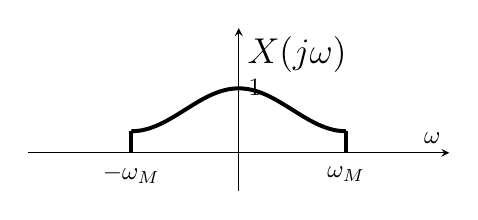
\begin{tikzpicture}[scale=0.9,transform shape]
    \begin{axis}[
        x=0.05\textwidth,y=0.05\textwidth,
        axis y line=center,
        axis x line=middle,
        xlabel=$\omega$,ylabel={\Large $X(j\omega)$},
        xmin=-4.9,xmax=4.9,
        ymin=-0.9,ymax=2.9,
        ticks=none
        ]
        \addplot [
        black, ultra thick,
        domain=-2.5:2.5, smooth
        ] {cos(deg(2*pi/5*x))*.5+1} ;
        \addplot [
        black, ultra thick
        ] coordinates {(-2.5,0) (-2.5,.5)} ;
        \addplot [
        black, ultra thick
        ] coordinates {(2.5,0) (2.5,.5)} ;
        \node at (-2.5,-.5) {$-\omega_M$};
        \node at (2.5,-.5) {$\omega_M$};
        \node at (0.15,1.5) {$\mathbf{-}1$} ;
    \end{axis}
    \end{tikzpicture}